\documentclass[a4paper,11pt]{scrartcl}
\usepackage[utf8x]{inputenc}
\usepackage[catalan]{babel}
\usepackage{titlesec}
% A ses llengües llatines, el primer paràgraf ha d'anar tabulat
\usepackage{indentfirst}
\usepackage{amsmath}
\usepackage{float}
\usepackage{graphicx}
\usepackage{subfigure}
\usepackage{booktabs}
\usepackage{multirow}
\usepackage{hyperref}
\usepackage{url}
\usepackage{multirow}
\usepackage{tabularx}

%% apt-get install python-pygments
%% wget http://minted.googlecode.com/hg/minted.sty
\usepackage{minted} %

%% aptitude install texlive-fonts-extra
\usepackage{newcent} %font mes wapa

\graphicspath{{diagrames/}}

% Estil de seccions
\titleformat{\section}{\large\sectfont}{\thesection}{1em}{}
\titleformat{\subsection}{\bfseries\sectfont}{\thesubsection}{1em}{}
% Estil numeracio subseccions http://help-csli.stanford.edu/tex/latex-sections.shtml#number
%\def\thesubsection{\alph{subsection})}

%% Tamany del codi font python inserit amb el minted
\newcommand{\codeSize}{\footnotesize}

\title{Pràctica de Cerca Local: \\ \huge{Carmageddon}}
\author{ Miquel Mas Fiol \thanks{mkelmas a gmail punt com} \\
	 Bartomeu Miró Mateu \thanks{bartomeumiro a gmail punt com} \\}

\begin{document}

  \maketitle

  \begin{abstract}
    \begin{center}
      
\includegraphics[width=0.6\textwidth]{figures/carmageddon-logo.png}
    \end{center}
  \end{abstract}

  \newpage
  \setcounter{page}{2}
  \tableofcontents
  \newpage

  \section{Interpretació de l'enunciat}

En aquest problema tenim una ciutat, passatgers i conductors. Tots els passatgers i conductors
tenen un origen i un destí fixat dins la ciutat on han d'arribar i volem sabre quins conductors
transporten a quins passatgers, sabent la ruta que duen a terme.

Tots els passatgers poden ser recollits per un conductor que el portarà al seu destí,
així doncs un passatger no pot fer el seu trajecte amb més de un conductor.

Hem de tenir amb compte que els conductors tenen una capacitat \emph{C} limitada del vehicle que no pot ser
sobrepassada. Això significa que en un mateix instant no hi pot haver més de \emph{C} passatgers dins un vehicle,
no obstant durant tot el recorregut del conductor pot deixar i recollir diversos passatgers arribant a transportar
més de \emph{C} passatgers\cite{maxCapaDepenentDeRuta}.

\begin{center}[H] \ref{maxCapaDepenentDeRuta}
 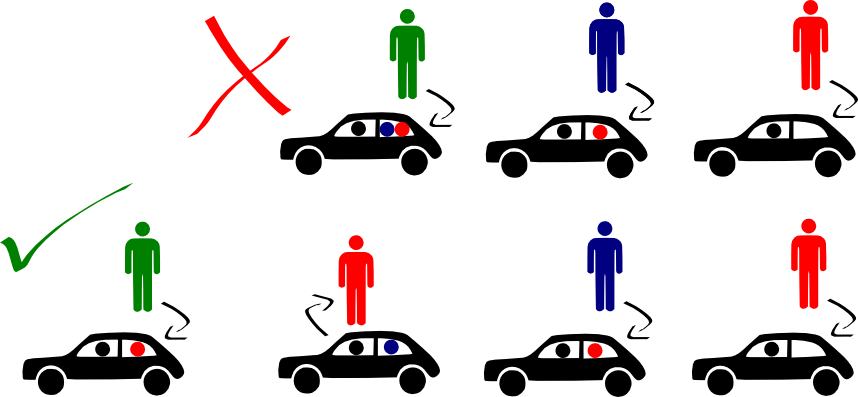
\includegraphics[width=0.6\textwidth]{figures/maxCapaDepenentDeRuta.png}
\end{center}


\emph{Tots} els conductors i passatgers han d'arribar \textbf{a temps} al seu destí. Donat que és
suposa una velocitat \emph{V} constant i que el conductor és l'últim arribar això significa aquest no podrà
superar més d'una determinada distància. En concret es presenta l'escena d'iniciar la ruta a les 7 del mati
i acabar a les 8. Això dona una hora recorregut a velocitat V per el conductor. Si aquesta velocitat es
de 30km/h tenim que un conductor pot recórrer com a molt 30km en la seva ruta. Notem que en l'àmbit
d'aquest problema suposam que el cost temporal de pujar o baixar un passatger és despreciable.

Un conductor pot passar a ser passatger. En tal cas es comportarà com un passatger més. Dit cas
dependrà de la valoració que es faci d'eliminar un conductor o de si comparteix ruta amb un altre
conductor amb espai lliure i que per tant així es minimitza la distància recorreguda.

Donat aquest escenari tenim dos criteris de minimització.
Per una banda volem minimitzar \textbf{la distància total recorreguda} per tots els conductors i per l'altra
a més de minimitzar la distància també volem minimitzar el \texttt{número de conductors}.

Hem de tenir amb compte que dins el primer en certa mesura també s'inclou la minimització de conductors
ja que el còmput de distància es fa per número de conductors i en cas d'haver dos conductors compartint
ruta el fet d'eliminar-ne un resta la distància de la seva ruta minimitzant el còmput total.

En quan al segon criteri s'ha de preveure que número de conductors i kilòmetres són dues unitats de 
mesura diferents que han de donar lloc a una única valoració per tant s'haurà d'establir una manera 
de combinar-les o cercar-hi alguna relació.

\section{Paràmetres}

El número de persones total ve determinat per el paràmetre $N$, de les quals $M$ no són conductors,
son passatgers, així doncs el numero de conductors es $N-P$. 

La ciutat és defineix com una matriu de 10x10 Km on cada illeta es de 100x100 m, així doncs
la ciutat és una matriu de 100x100 illetes.

La distància \emph{D} entre punts (\emph{o}rigen i \emph{d}estí) de la ciutat ve determinada per la funció:
$$ D(o,d) = |o_x - d_x| + |o_y - d_y| $$

Hem de tenir amb compte que la ciutat al ser una matriu per anar d'un punt A a un punt B hi ha múltiples
rutes amb la mateixa distància. Cosa que pot suposar un avantatge ja que així els únics paràmetres
d'una ruta son el punt d'origen, el destí i la distància.

  \newpage
  \section{Modelització del problema}

\subsection{Representació de les dades}
\subsubsection{Ciutat}
\subsubsection{Passatger}
\subsubsection{Conductor}
\subsubsection{Estat}

\subsection{Estat inicial}


\subsection{Operadors de transformació}


\subsection{Heurístic}
  \newpage
  \section{Experimentació}

\subsection{Se\lgem ecció dels operadors}

\subsection{Se\lgem ecció de la generació de l'estat inicial}

\subsection{Se\lgem ecció dels paràmetres del Simulated Anealing}
Per a determinar els paràmetres que obtenen un millor resultat per a l'execució de l'algorisme \emph{simulated annealing},
hem executat reiterades vegades l'algorisme amb diferents parametres per a \texttt{lambda} i \texttt{k}, concretament s'ha fet amb
\texttt{[0.1,0.01,0.001,0.0001]} i \texttt{[1,5,25,125]} repectivament, fixant el nombre d'iteracions en 2000.

El millor resultat s'ha obtingut amb els parametres [p1] [p2], com indica el seguent grafic.

(GRAFIC)

Fixats aquests dos paràmetres en els valors que han obtingut millor resultat, s'ha ajustat el nombre d'iteracions executant diverses 
vegades l'algorisme amb un nombre diferent d'iteracions. Es pot veure en el seguent gràfic el millor valor per al nombre d'iteracions.



(GRAFIC)

Aleshores, podem comparar els resultats obtinguts amb simulated Annealing i Hill climbing.

Per una banda pot observar que el simulated Annealing obté un resultat menys costós en termes de nombre de quilometres de la solucio,
 pero amb un cost temporal mes elevat.

(GRAFIC)

(GRAFIC)


\subsection{Observació de l'evolució temporal del Hill Climbing}

\subsection{Se\lgem ecció dels valors de ponderació del segon heurístic}

\subsection{Se\lgem ecció del valor de \emph{M} per millor inicialització del problema}
  \newpage
  \section{Manual d'usuari}

La practica està escrita en \emph{python}\footnotemark, per tant és necessari tenir
l'interpret insta\lgem at.
Es recomana l'ús de \emph{pypy}\footnotemark en lloc de l'interpret per defecte ja 
que aquest implementa un \emph{just-in-time complier} i accelera notablement l'execució
de la pràctica.

Per dur a terme l'execució s'ha de fer amb el fitxer \texttt{prog.py} si es executat
sense parametres mostrarà quins suporta i alguns exemples d'execució.

Essencialment te dues maneres de funcionar, una es executar un test dels demanats a l'enunciat,
l'altre es executar un hill climbing o simulated anealing amb determinats paràmetres.

\subsection{Execució d'un test}
Per executar un test simplement s'ha de passar com a paràmetre el número del test a executar i 
aquest s'executara i mostrarà per pantalla el resultat.

En cas que sigui un test amb diferents opcions per defecte s'executa amb la opció que dona
una millor execució. Per tal de canviar dites opcions s'ha d'editar el fitxer prog.py anant
a la capçalera de la funció i canviant el paràmetre per defecte.

\begin{minted}[fontsize=\small]{python}
def test4_TemporalEvolution(operatorSet="1", initDistrib="allOneFirst"):
   ...
\end{minted}

\subsection{Execució simple}
Si sols volem executar una una cerca simple tenim dues opcions, una es carregar un fitxer de configuració
guardat i l'altre espeficicar tots els paràmetres.

Els paràmetres per a fer una execució simple són:

\begin{minted}[fontsize=\small]{bash}
pypy prog.py N M inicialitzacio heuristic conjuntOperadors algorismeCerca

\small
\begin{center}
\begin{tabularx}{\textwidth}{llX}
\textbf{parametre}  & \textbf{Valors} & \textbf{Descripció}\\
\midrule
N  & valor enter & Numero d'usuaris del servei\\
M  & valor enter & NUmero d'usuaris no conductors\\
\midrule
inicialització & allOneFirst & REF\\
               & fullFirst   & REF\\
\midrule
heuristic      & km  & Minimitza el número de km recorreguts\\
	       & veh & Mínimitza el numero de km i el numero de conductors\\
\midrule
conjuntOperadors      & 1 & Moure passatgers i llevar conductors buits\\
		      & 2 & Intercanviar passatgers i llevar conductors\\
\midrule
algorismeCerca & hillClimbing & Executa un Hill Climbing\\
               & simulatedAnnealing & Executa Simulated Annealing
\end{tabularx}
\end{center}
\normalsize


Els paràmetres per fer una execució des de un fitxer són:

\begin{minted}[fontsize=\small]{bash}
pypy prog.py fitxer.cfg heursistic conjuntOperadors algorismeCerca
\end{minted}

On fitxer es el nom del \texttt{fitxer.cfg} de configuració i la resta de paràmetres són
iguals a l'apartat anterior.

\footnotetext{\url{http://python.org}}
\footnotetext{El lloc oficial és \url{http://pypy.org/} però es pot
trobar precompilat i empaquetat per Debian/Ubuntu a \url{https://launchpad.net/~pypy/+archive/ppa}}


  \newpage
   \let\thefootnote\relax\footnotetext{
 Aquest document està baix llicència \href{http://creativecommons.org/licenses/by-sa/3.0/}{Creative Commons Atributive Share-Alike 3.0}
 per tant es pot compartir, modificar i distribuir, però citant els autors originals i sense modificar la llicència.
 De la mateixa manera el codi font està baix llicència GNU GPL v3 per part dels dos autors.\bigskip}
\let\thefootnote\relax\footnotetext{El document en versió digital i el codi font el trobareu a \\
\url{https://github.com/bmiro/carmageddon}\bigskip}
\let\thefootnote\relax\footnotetext{Aquest document i tota la part de la pràctica ha estat desenvolupat emprant programari lliure:}
\let\thefootnote\relax\footnotetext{\href{http://www.tug.org/applications/pdftex/}{\LaTeX} i \href{http://www.tug.org/applications/pdftex/}{Kile} per el text,
\href{http://www.inkscape.org/}{Inkscape} pels diagrames,
\href{http://kate-editor.org/}{Kate} i \href{http://vim.org/}{Vim} per l'edició del codi font.
\href{http://git-scm.com/}{Git} com a sistema de control de versions.
\href{http://python.org/}{Python} com a llenguatge de programació.
}

\let\thefootnote\relax\footnotetext{
\begin{center}
\begin{tabular}{cc}

\includegraphics[height=35pt,keepaspectratio=true]{diagrames/by-sa.png}
 & 
\includegraphics[height=35pt,keepaspectratio=true]{diagrames/gnu.png}
\end{tabular}
\end{center}
\begin{center}
\begin{tabular}{cccccc}
 
\includegraphics[height=35pt,keepaspectratio=true]{diagrames/latex.png}
 & 
\includegraphics[height=35pt,keepaspectratio=true]{diagrames/kile.png}
 & 
\includegraphics[height=35pt,keepaspectratio=true]{diagrames/inkscape.png}
 & 
\includegraphics[height=35pt,keepaspectratio=true]{diagrames/vim.jpg}
 & 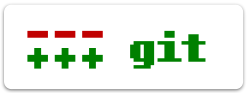
\includegraphics[height=35pt,keepaspectratio=true]{diagrames/git.png}
 & 
\includegraphics[height=35pt,keepaspectratio=true]{diagrames/python.png}
\end{tabular}
\end{center}
}

  \newpage

  \section{Annex: Codi font}

\subsection{Carmageddon}
\inputminted[linenos, frame=lines, fontsize=\codeSize]{python}{../aima/carmageddon.py}
\newpage

\subsection{State}
\inputminted[linenos, frame=lines, fontsize=\codeSize]{python}{../aima/state.py}
\newpage

\subsection{Driver}
\inputminted[linenos, frame=lines, fontsize=\codeSize]{python}{../aima/driver.py}
\newpage

\subsection{Passenger}
\inputminted[linenos, frame=lines, fontsize=\codeSize]{python}{../aima/passenger.py}
\newpage


\subsection{showLog}
\inputminted[linenos, frame=lines, fontsize=\codeSize]{python}{../aima/showLog.py}


\subsection{Prog}
\inputminted[linenos, frame=lines, fontsize=\codeSize]{python}{../aima/prog.py}



\end{document}
